\documentclass[a4paper,10pt]{article}
%\usepackage[utf8x]{inputenc}

% Lay out packages
\usepackage[margin=3cm]{geometry}
\usepackage[utf8]{inputenc}
\usepackage{mathpazo}

\usepackage{amsmath}
\usepackage{graphicx}

% Dutch style of paragraph formatting, i.e. no indents. 
\setlength{\parskip}{1.3ex plus 0.2ex minus 0.2ex}
\setlength{\parindent}{0pt}

%opening
\title{Computer Vision Assignment 1: Filtering}
\author{Robrecht Jurriaans (5887380), Taco Cohen (6394590)}

\begin{document}

\maketitle


\section{Gaussian Filters}

\subsection{1D Gaussian Filter}
We implemented the 1D Gaussian in \verb+gaussian.m+.
We made sure the kernel size is about $3*\sigma$ and is always odd (using the \verb+ceil+ function).

Because the filter has a finite size, the sum of the filter values will not be one in a naive implementation.
For this reason, we must normalize the kernel after calculating the values of the Gaussian at each kernel entry.
To save computation, we used the following equality:

\begin{align*}
 \frac{G_{\sigma}(x)}{\sum_{x'=-h}^h G_{\sigma}(x')} &= \frac{ \frac{1}{\sigma \sqrt{2 \pi}} \exp(-\frac{x^2}{2 \sigma^2})}
       {\sum_{x'=-h}^h \frac{1}{\sigma \sqrt{2 \pi}} \exp(-\frac{x'^2}{2 \sigma^2})} \\
&= \frac{ \exp(-\frac{x^2}{2 \sigma^2})}
       {\sum_{x'=-h}^h \exp(-\frac{x'^2}{2 \sigma^2})}
\end{align*}

That is, we leave out the normalization of each index, because it falls out in the normalization of the entire kernel anyway.


\subsection{Convolving an image with a 2D Gaussian}
We implemented this the obvious way, relying on \verb+conv2+ to convolve the image first with the 1D x-direction filter, and then with the 1D y-direction filter.

\subsection{Comparing with Matlab's Gaussian Filter}
Thanks to the inherent separability of Gaussians, the implementation that convolves on one dimension at a time is slightly faster than the normal 2D implementation. We expect this difference to increase on larger images, as the difference is one of $O(N^2)$ versus $O(N)$. We note that there is a slight difference, on the order of $10^{-17}$ sum of squared differences, between the resulting images. This is likely due to rounding errors.

\begin{figure}[ht]
\begin{minipage}[b]{0.45\linewidth}
\centering
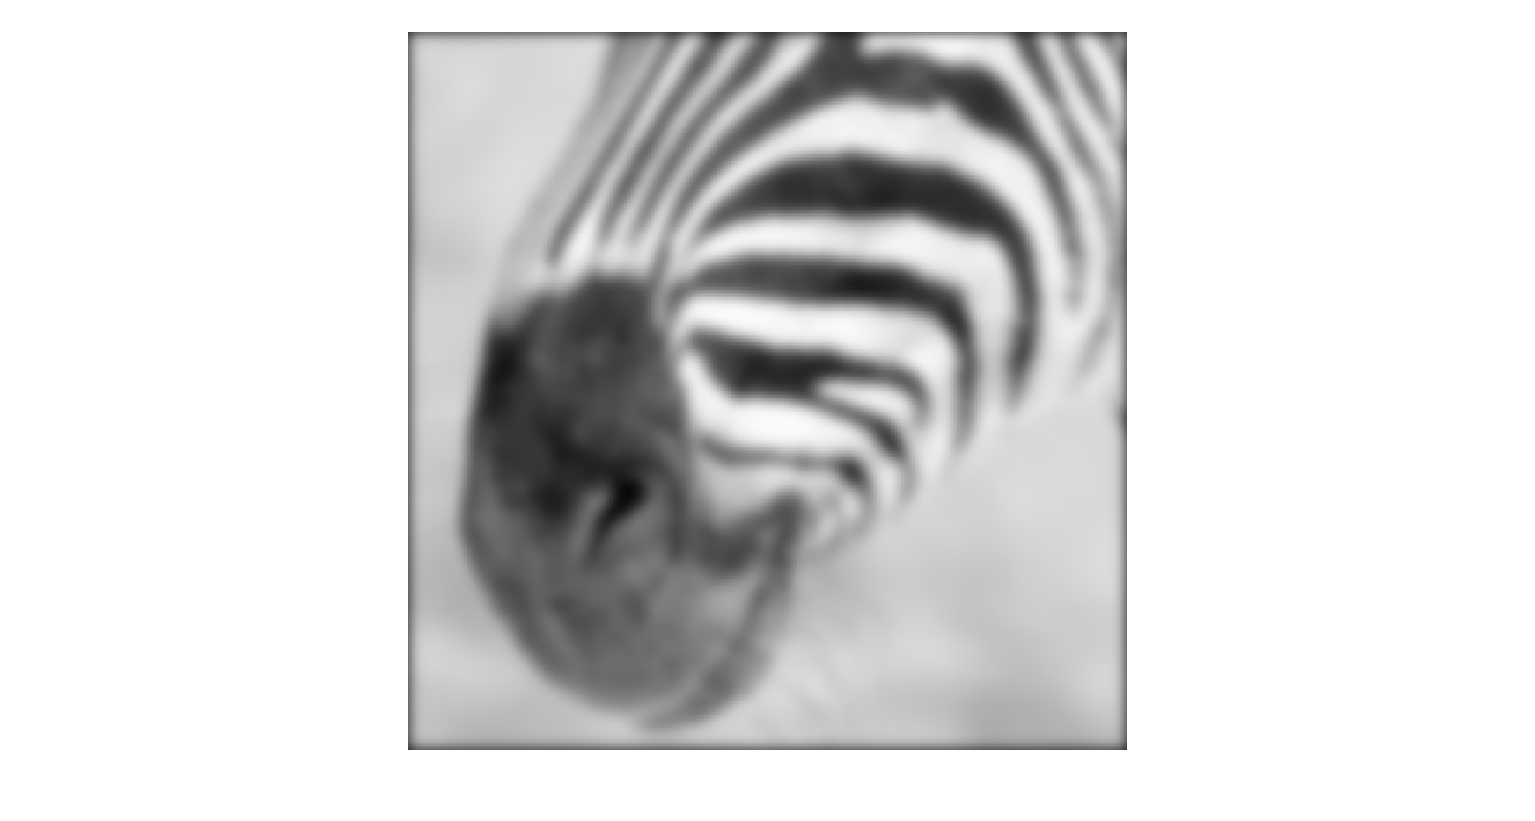
\includegraphics[width=\textwidth]{zebra_img/matlabfilter}
\caption{Original Matlab Filter}
\end{minipage}
\hspace{0.1cm}
\begin{minipage}[b]{0.45\linewidth}
\centering
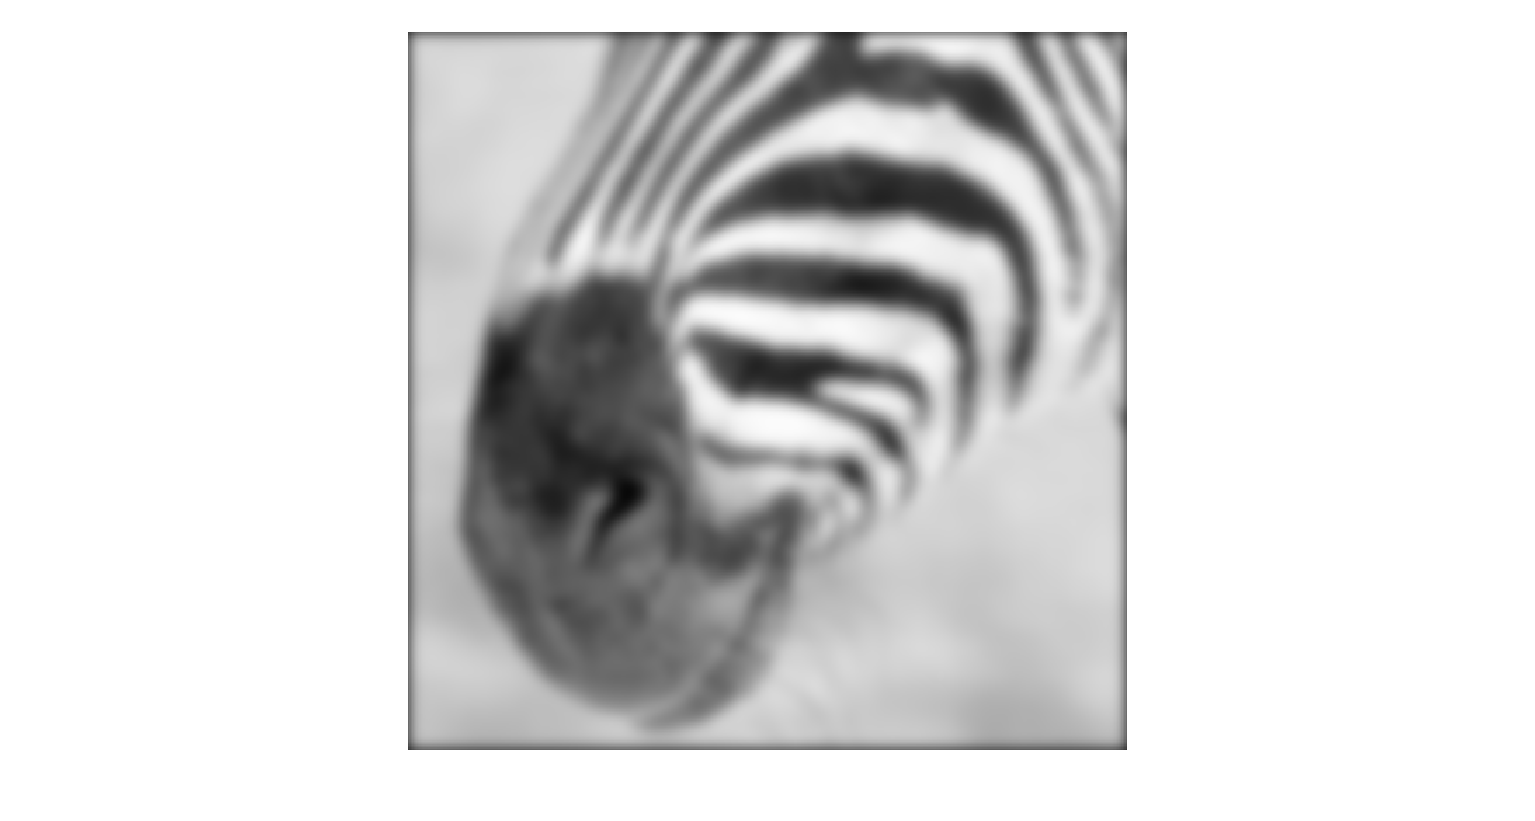
\includegraphics[width=\textwidth]{zebra_img/separatedfilter}
\caption{Filter based on separation}
\end{minipage}
\end{figure}

\subsection{Gaussian Derivative}
We implemented the Gaussian derivative, see \verb+GaussianDer.m+.

\subsection{Gradient Magnitude and Orientation}
We implemented the function \verb+gradmag+. The result is shown in the figures below.

\begin{figure}[ht]
\label{gradmag}
\begin{minipage}[b]{0.45\linewidth}
\centering
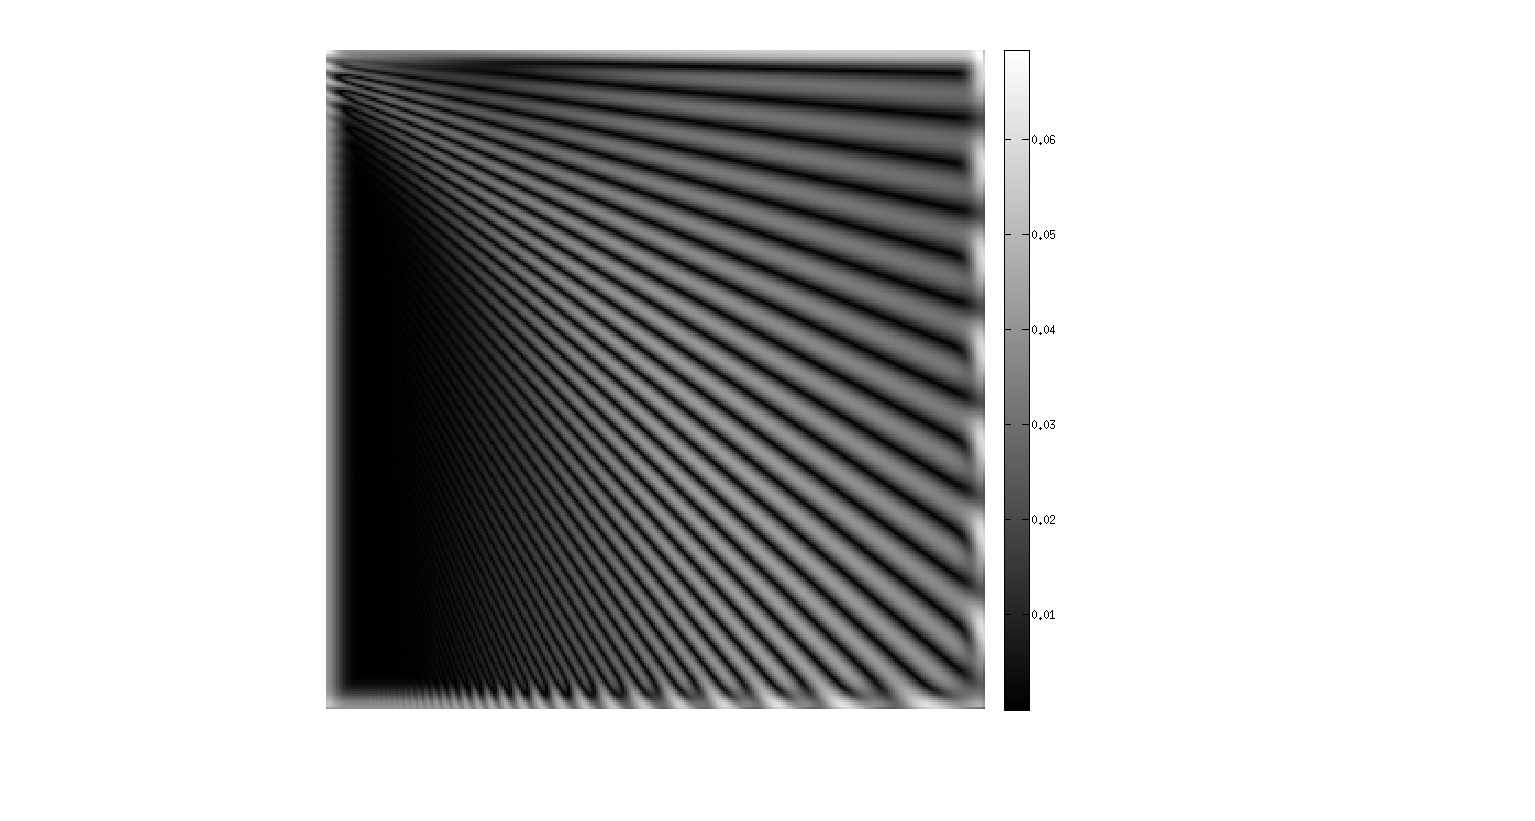
\includegraphics[width=\textwidth]{pn1_img/magnitude_sigma5_colorbar}
\caption{Magnitude image for $\sigma=5$}
\end{minipage}
\hspace{0.1cm}
\begin{minipage}[b]{0.45\linewidth}
\centering
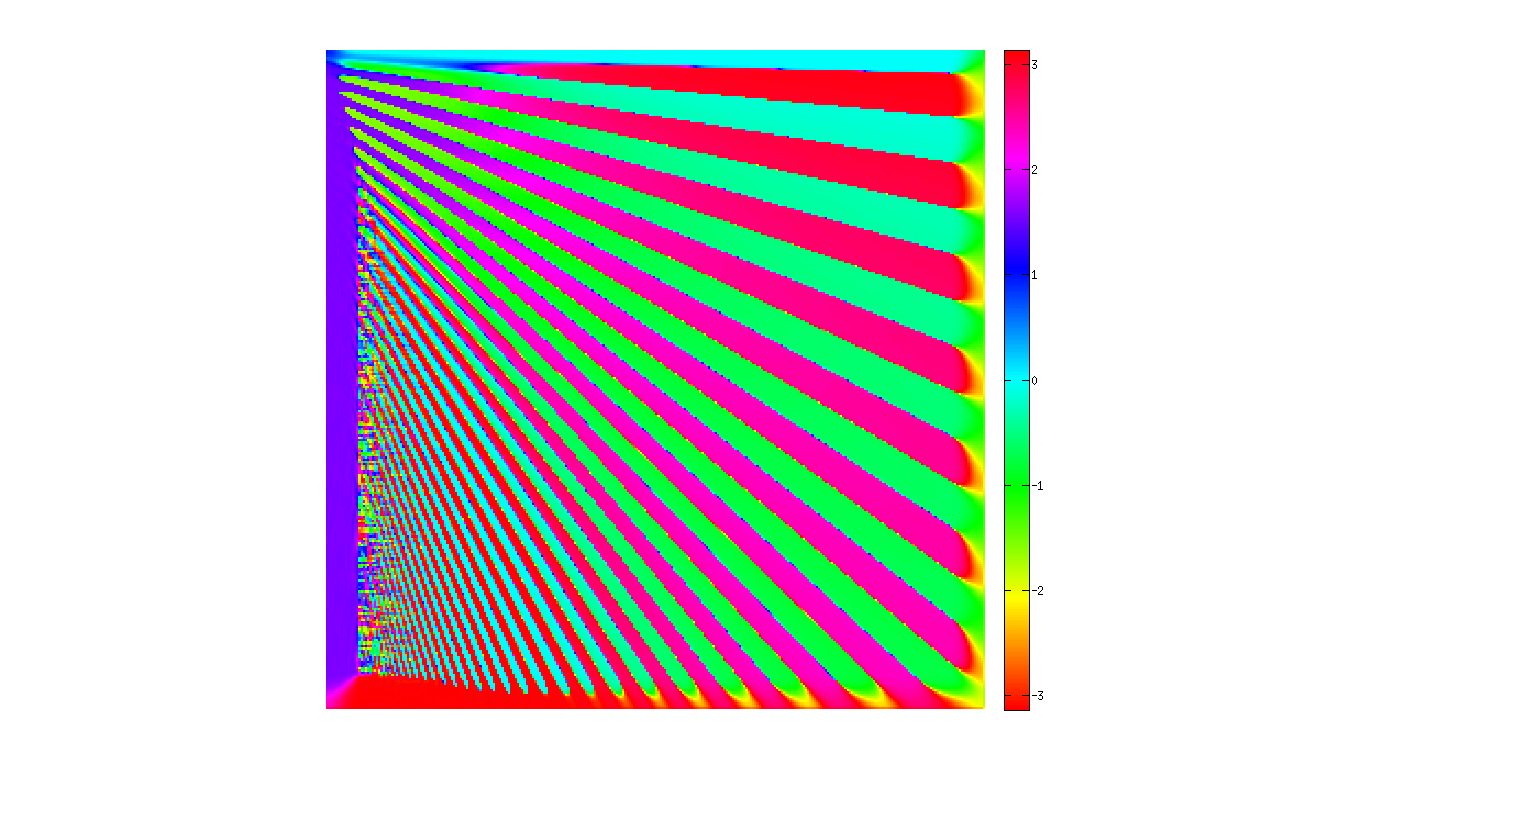
\includegraphics[width=\textwidth]{pn1_img/orientation_sigma5}
\caption{Orientation image for $\sigma=5$}
\end{minipage}
\end{figure}

\begin{figure}[ht]
\begin{minipage}[b]{0.45\linewidth}
\centering
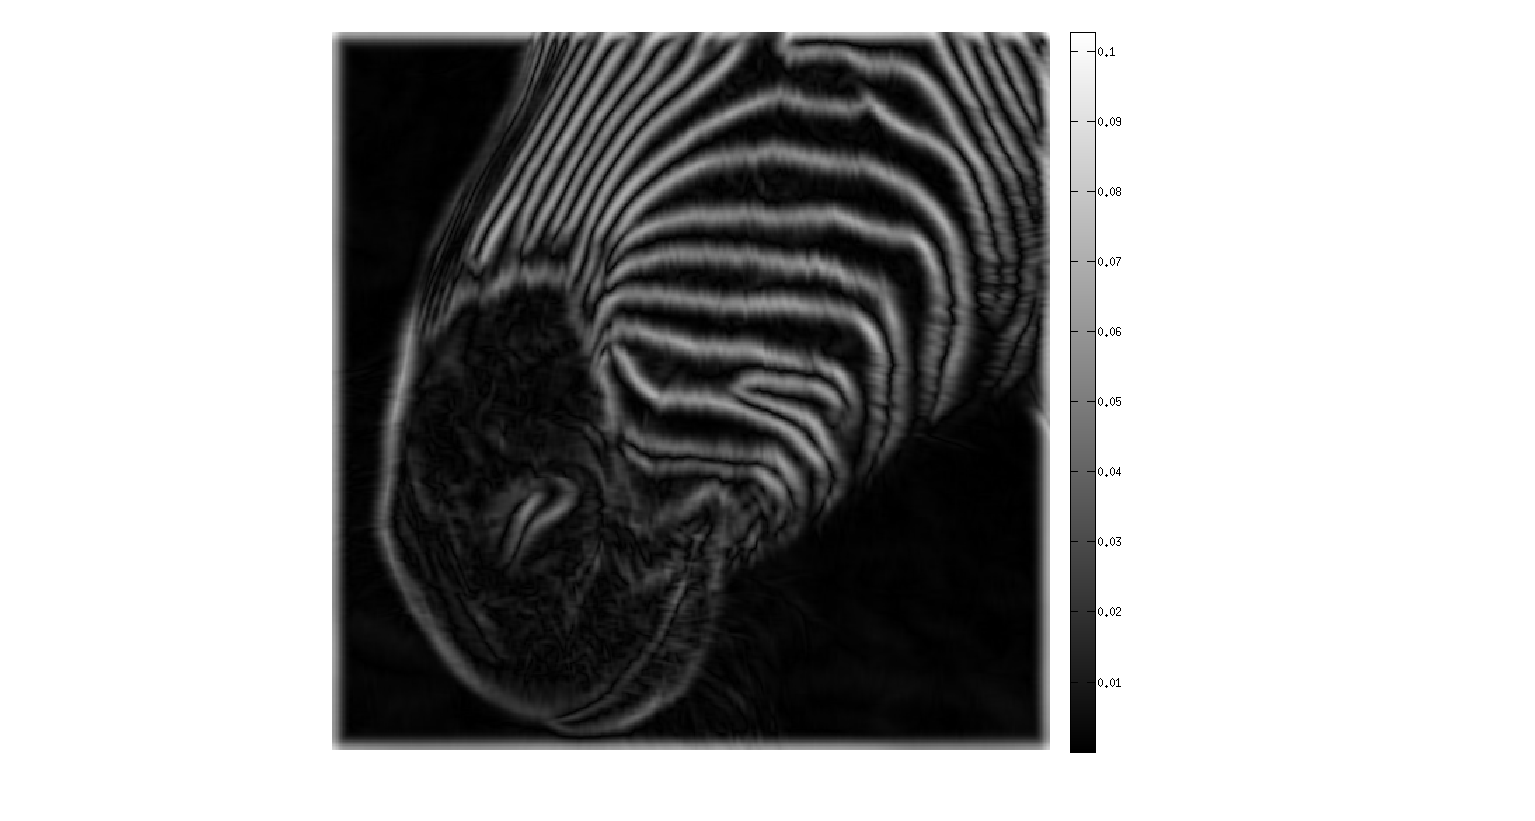
\includegraphics[width=\textwidth]{zebra_img/magnitude_sigma5_colorbar}
\caption{Magnitude image for $\sigma=5$}
\end{minipage}
\hspace{0.1cm}
\begin{minipage}[b]{0.45\linewidth}
\centering
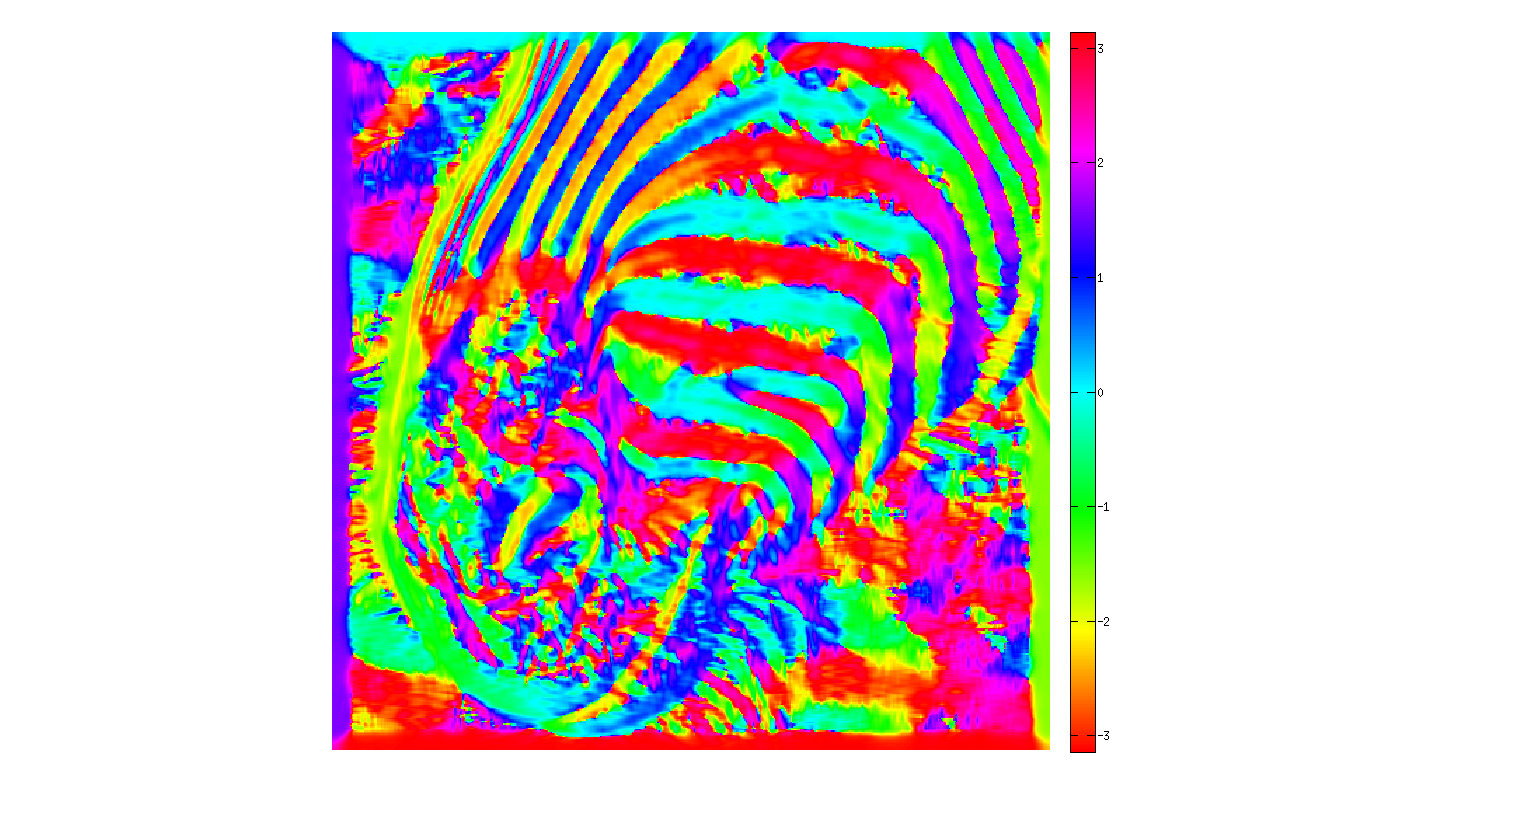
\includegraphics[width=\textwidth]{zebra_img/orientation_sigma5}
\caption{Orientation image for $\sigma=5$}
\end{minipage}
\end{figure}


\subsubsection{Quiver before my magnitude}
See the quiver plots below.

\begin{figure}[ht]
\centering
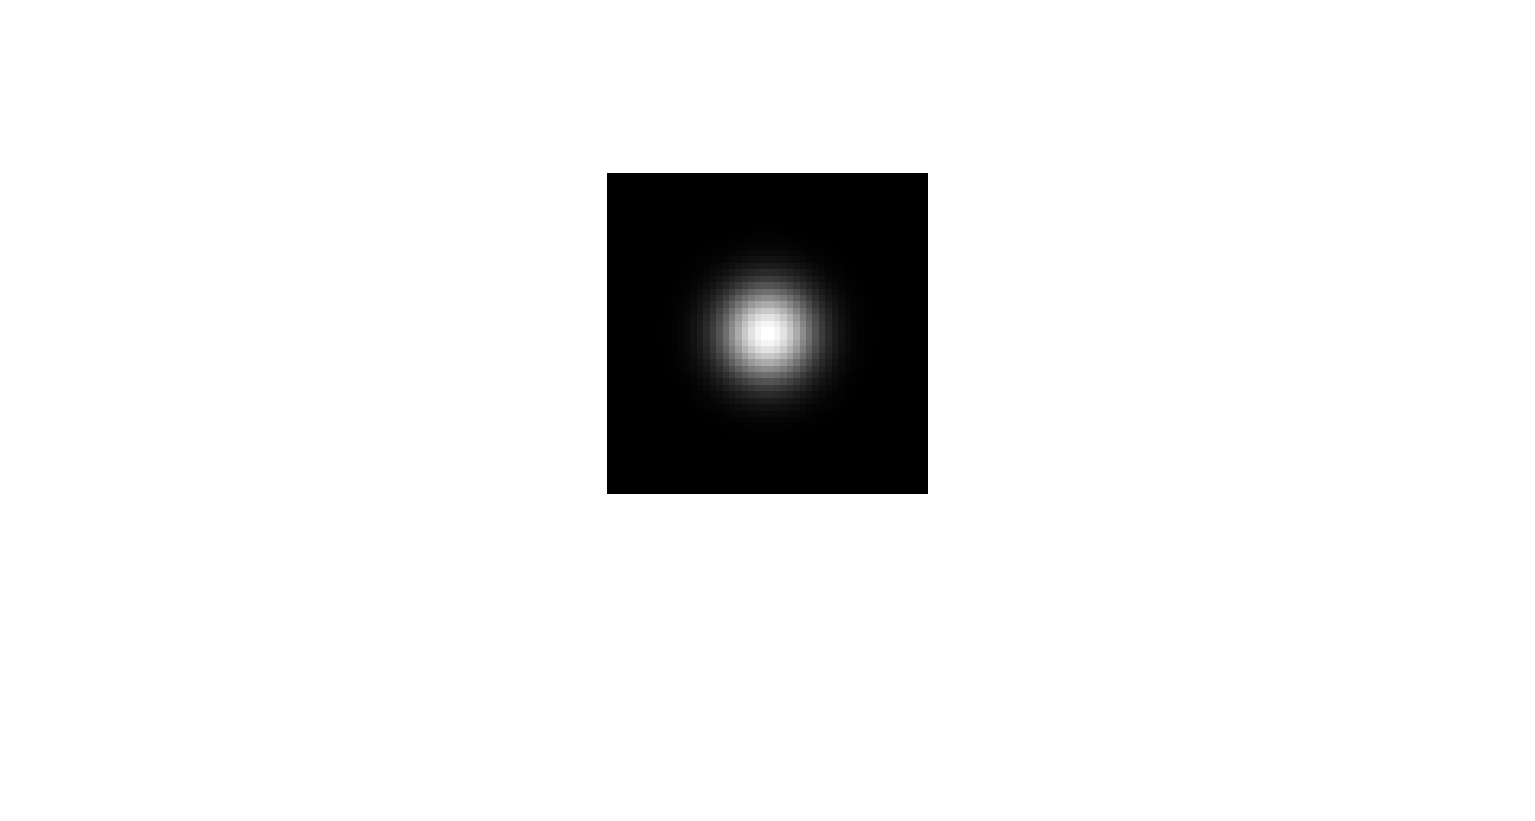
\includegraphics[width=\textwidth]{quiver_original}
\caption{Original image}
\label{fig:quiver_original}
\end{figure}
\begin{figure}[ht]
\begin{minipage}[b]{0.45\linewidth}
\centering
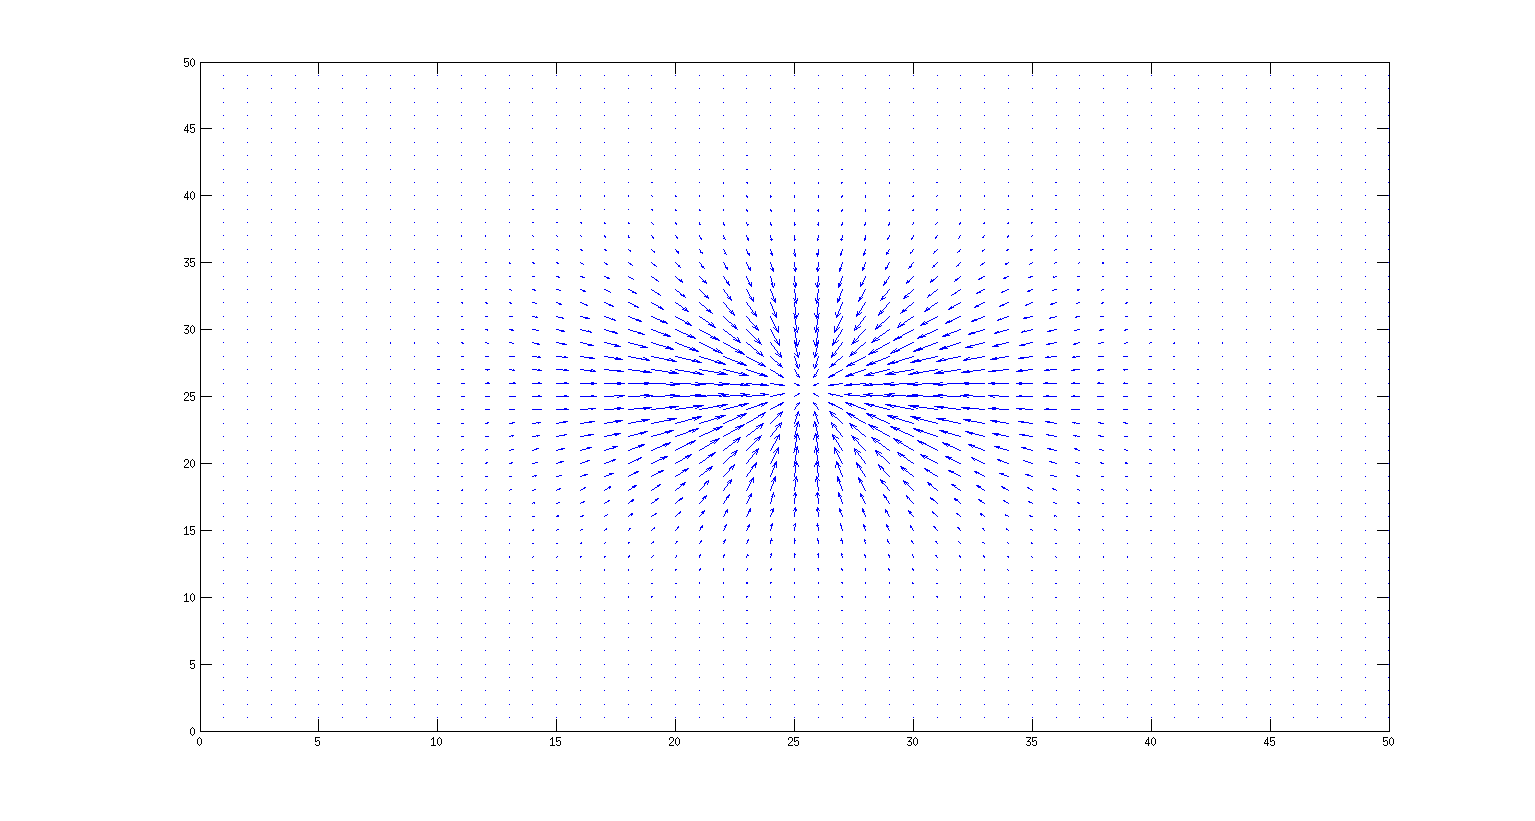
\includegraphics[width=\textwidth]{quiver_sigma1}
\caption{Gradient image for $\sigma=1$}
\end{minipage}
\hspace{0.1cm}
\begin{minipage}[b]{0.45\linewidth}
\centering
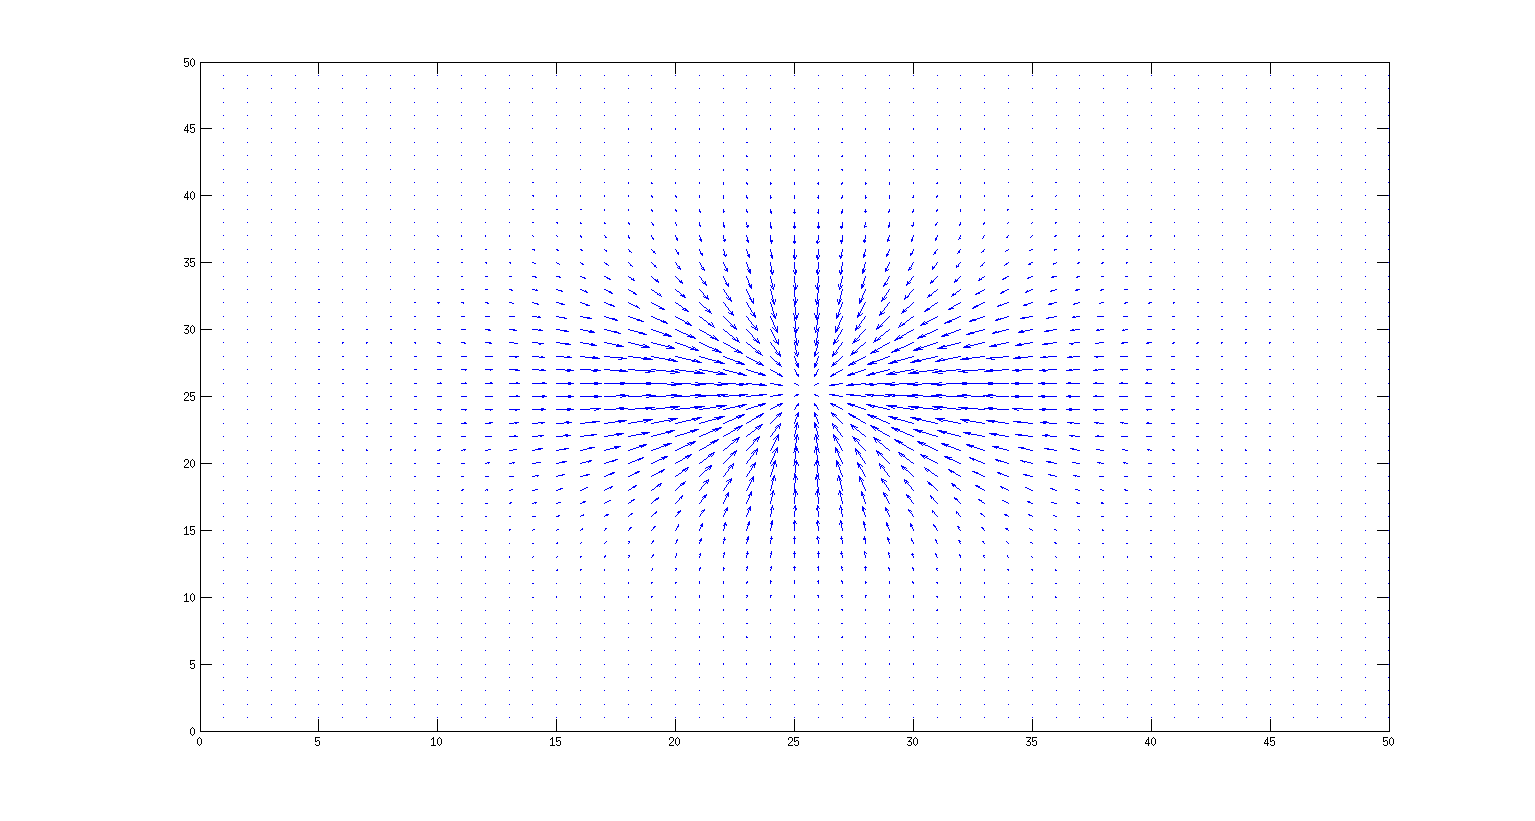
\includegraphics[width=\textwidth]{quiver_sigma3}
\caption{Gradient image for $\sigma=3$}
\end{minipage}
\end{figure}
\begin{figure}[ht]
\begin{minipage}[b]{0.45\linewidth}
\centering
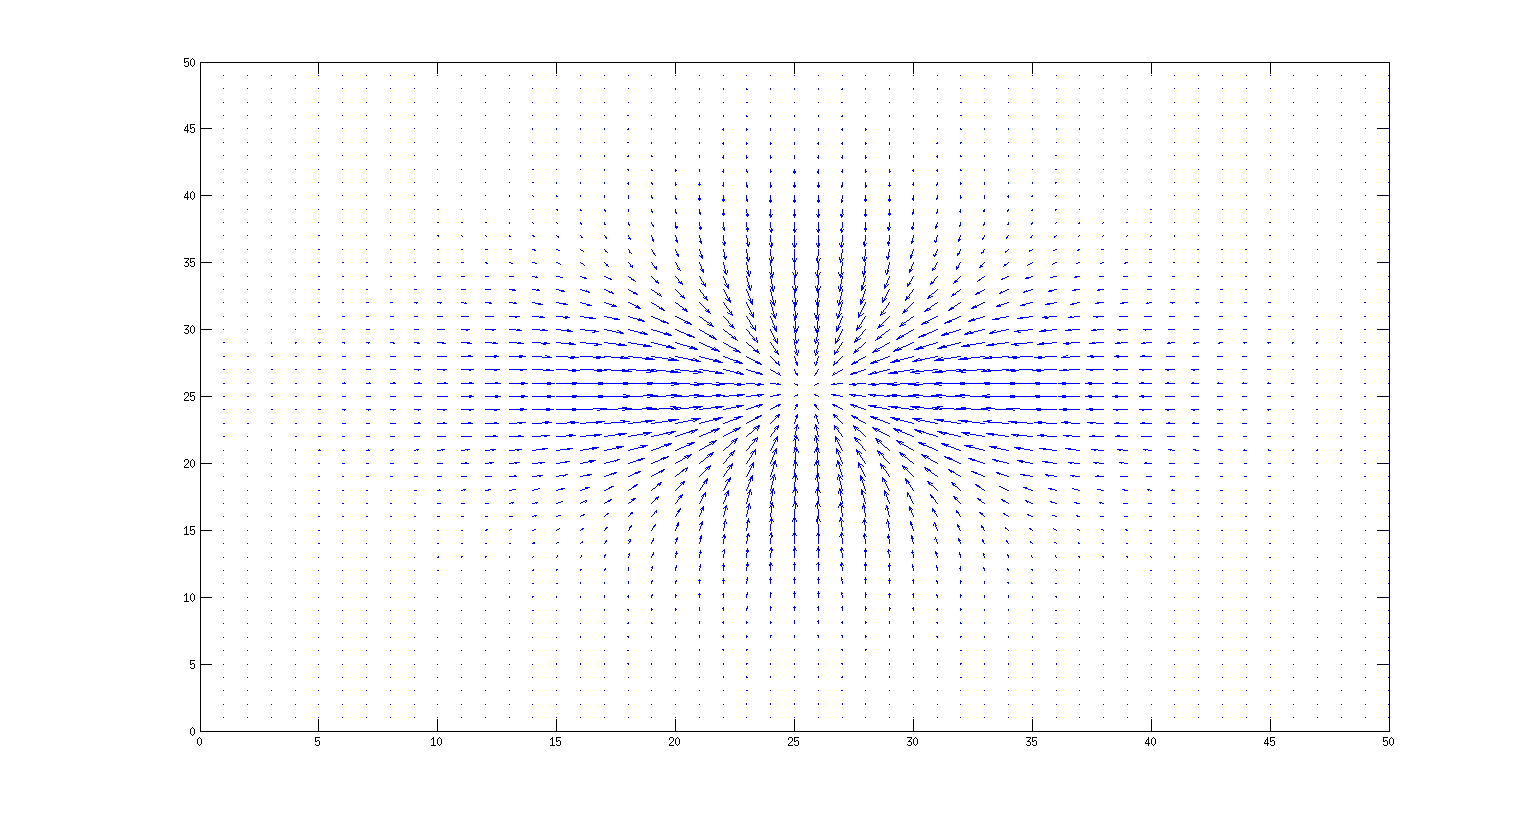
\includegraphics[width=\textwidth]{quiver_sigma5}
\caption{Gradient image for $\sigma=5$}
\end{minipage}
\hspace{0.1cm}
\begin{minipage}[b]{0.45\linewidth}
\centering
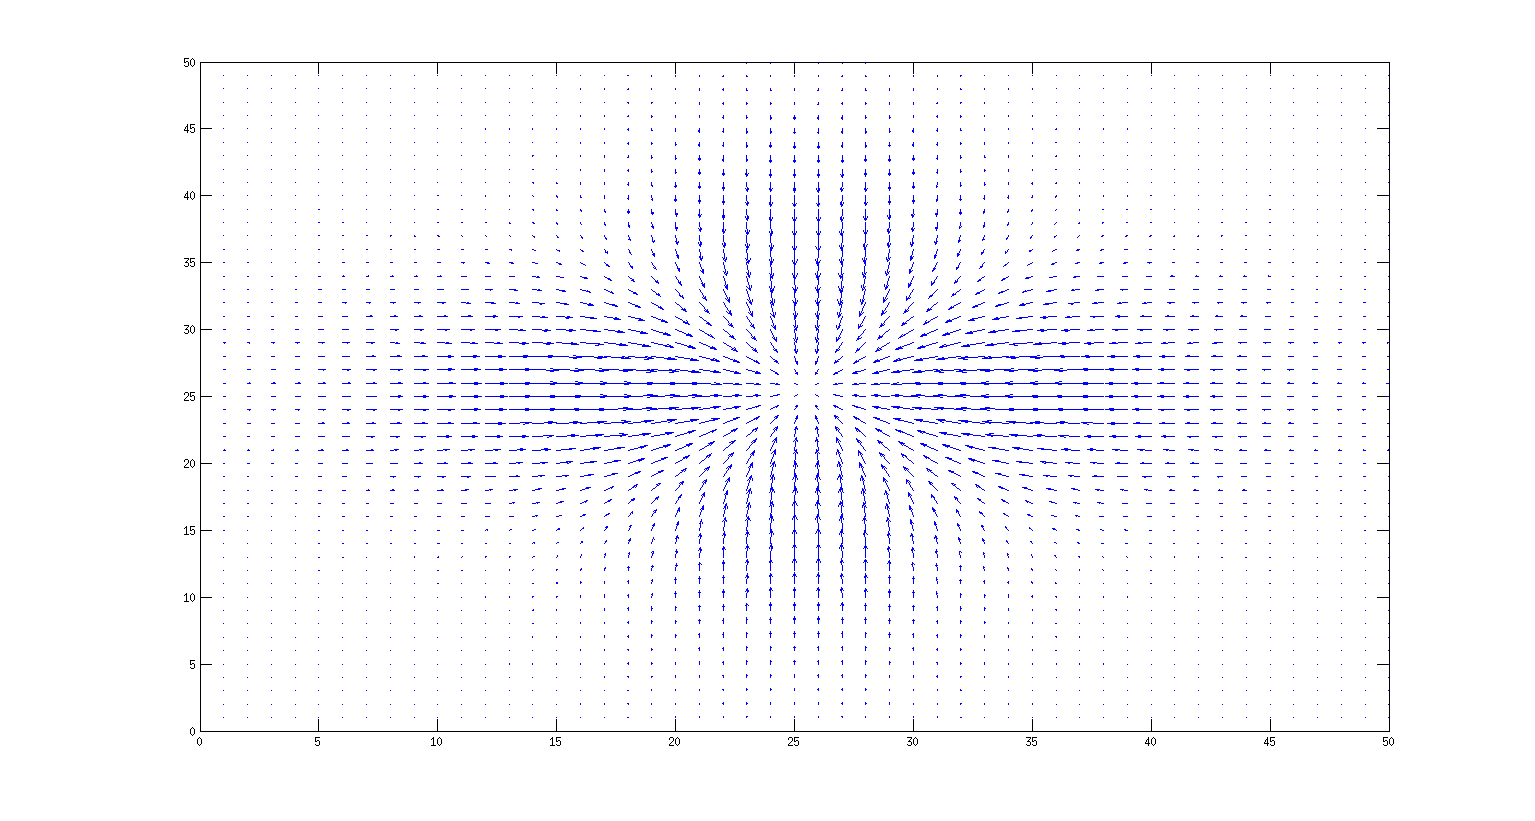
\includegraphics[width=\textwidth]{quiver_sigma7}
\caption{Gradient image for $\sigma=7$}
\end{minipage}
\end{figure}

\subsubsection{Magnitude and orientation for different $\sigma$}
Running \verb+master.m+ will result in gradient and orientation plots for various values of $\sigma$.
It is clear to see that for larger values of $\sigma$, only larger structures are retained.
The gradient is no longer affected by small details when $\sigma$ is large.
There is an obvious tradeoff here  between informativeness on small details and sensitivity to noise.
Likewise for the orientation plot.

\subsubsection{Threshold}
See figure \ref{fig:pn1thresh} for plots of thresholded gradient magnitudes for various thresholds and values of sigma.
\begin{figure}[ht]
\centering
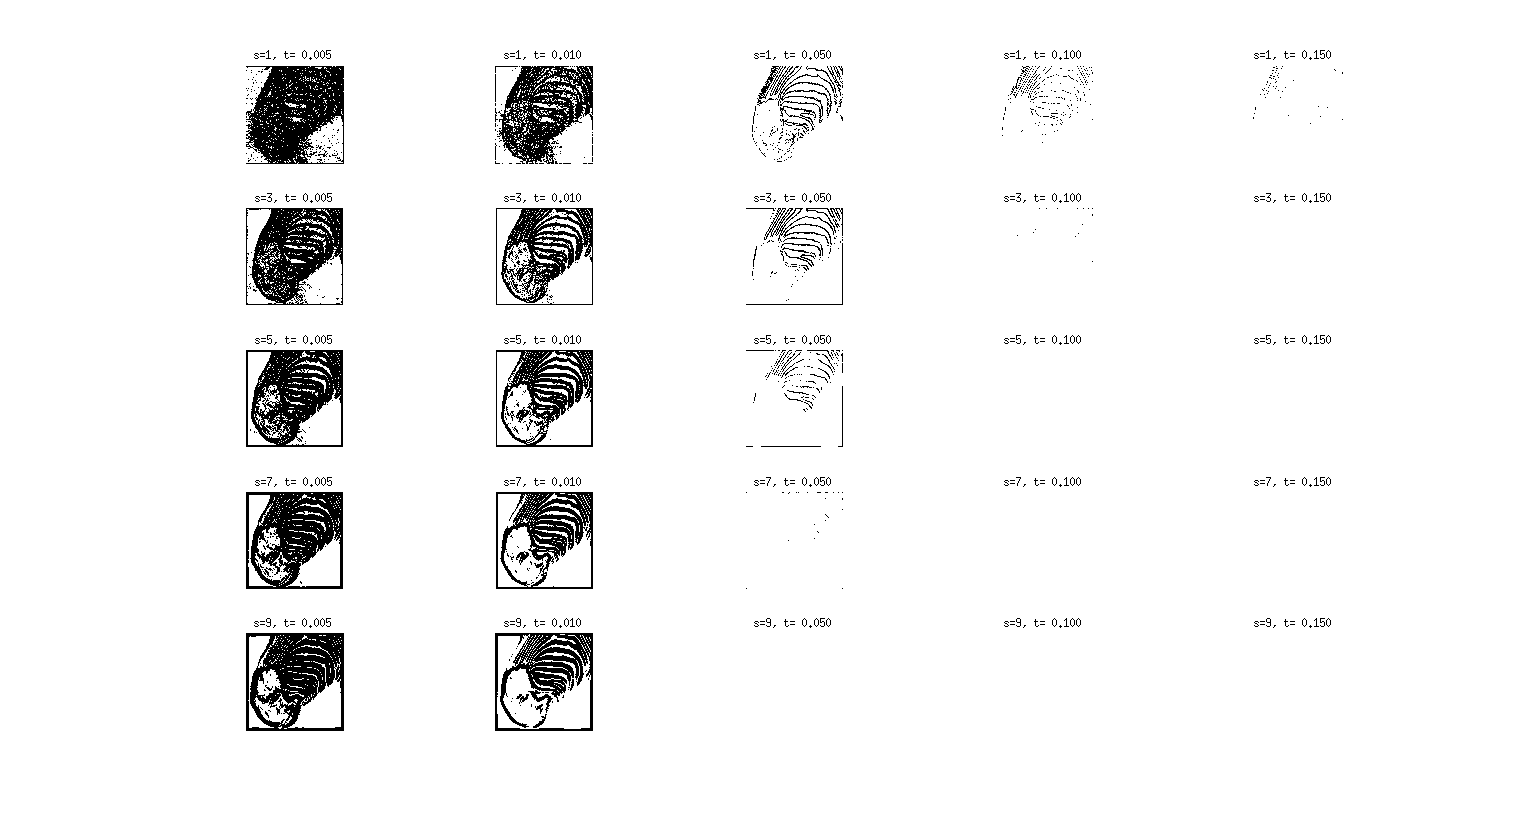
\includegraphics[width=\textwidth]{zebra_img/threshold}
\caption{Threshold images for various $\sigma$ and thresholds}
\label{fig:zebrathresh}
\end{figure}
\begin{figure}[ht]
\centering
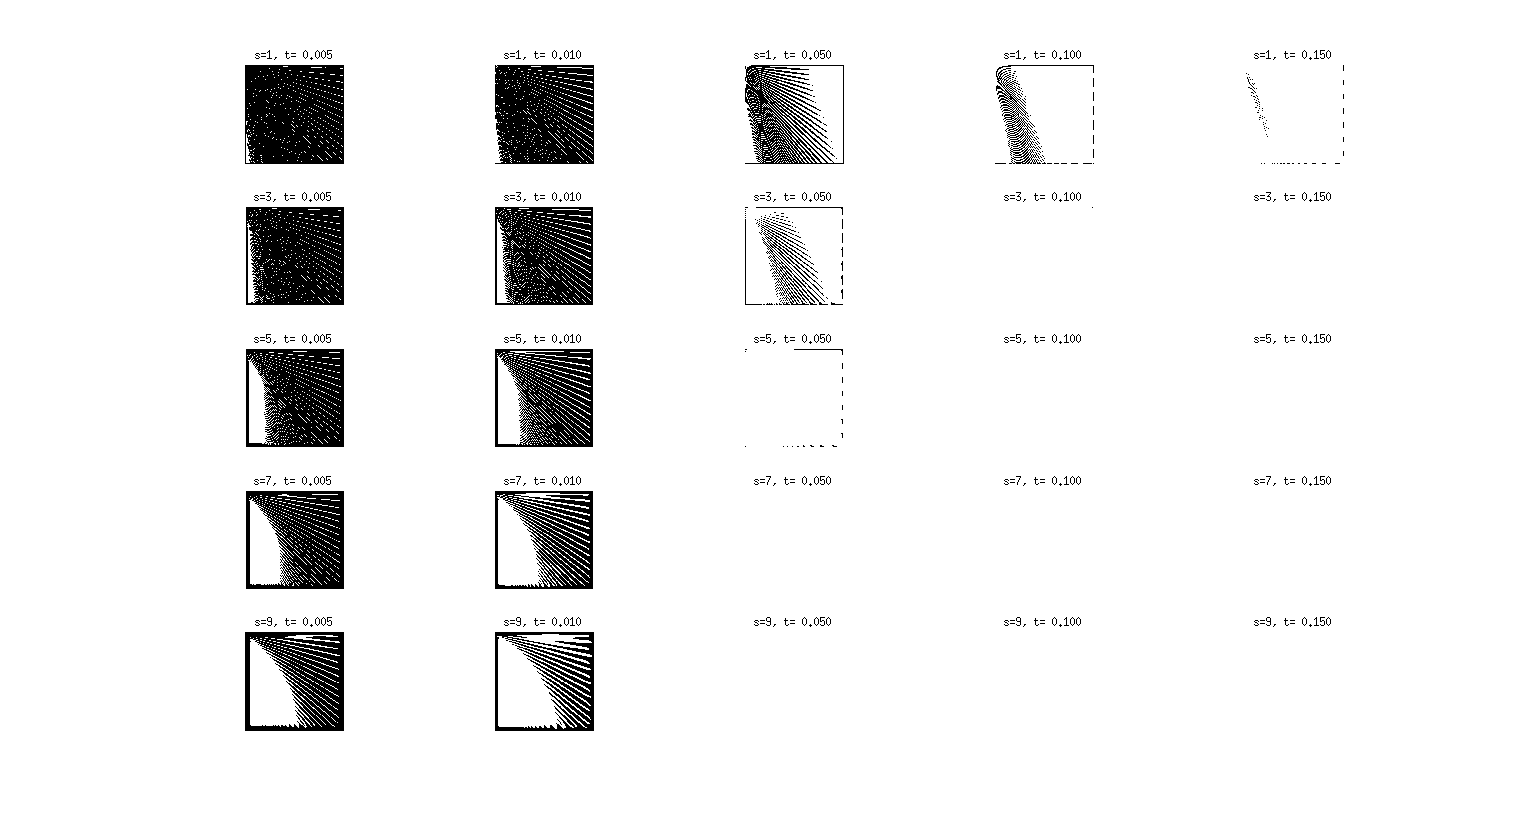
\includegraphics[width=\textwidth]{pn1_img/threshold}
\caption{Threshold images for various $\sigma$ and thresholds}
\label{fig:pn1thresh}
\end{figure}

\subsubsection{Second Order Derivative}
We implemented this function, see \verb+ImageDerivatives.m+.


\subsubsection{Impulse}
When convolving with an impulse, the response should be the filter.
This is what we see in figure \ref{fig:impulse}.
We notice that the shape of the kernel only depends on the order, while the size depends on the sigma.

\begin{figure}[ht]
\centering
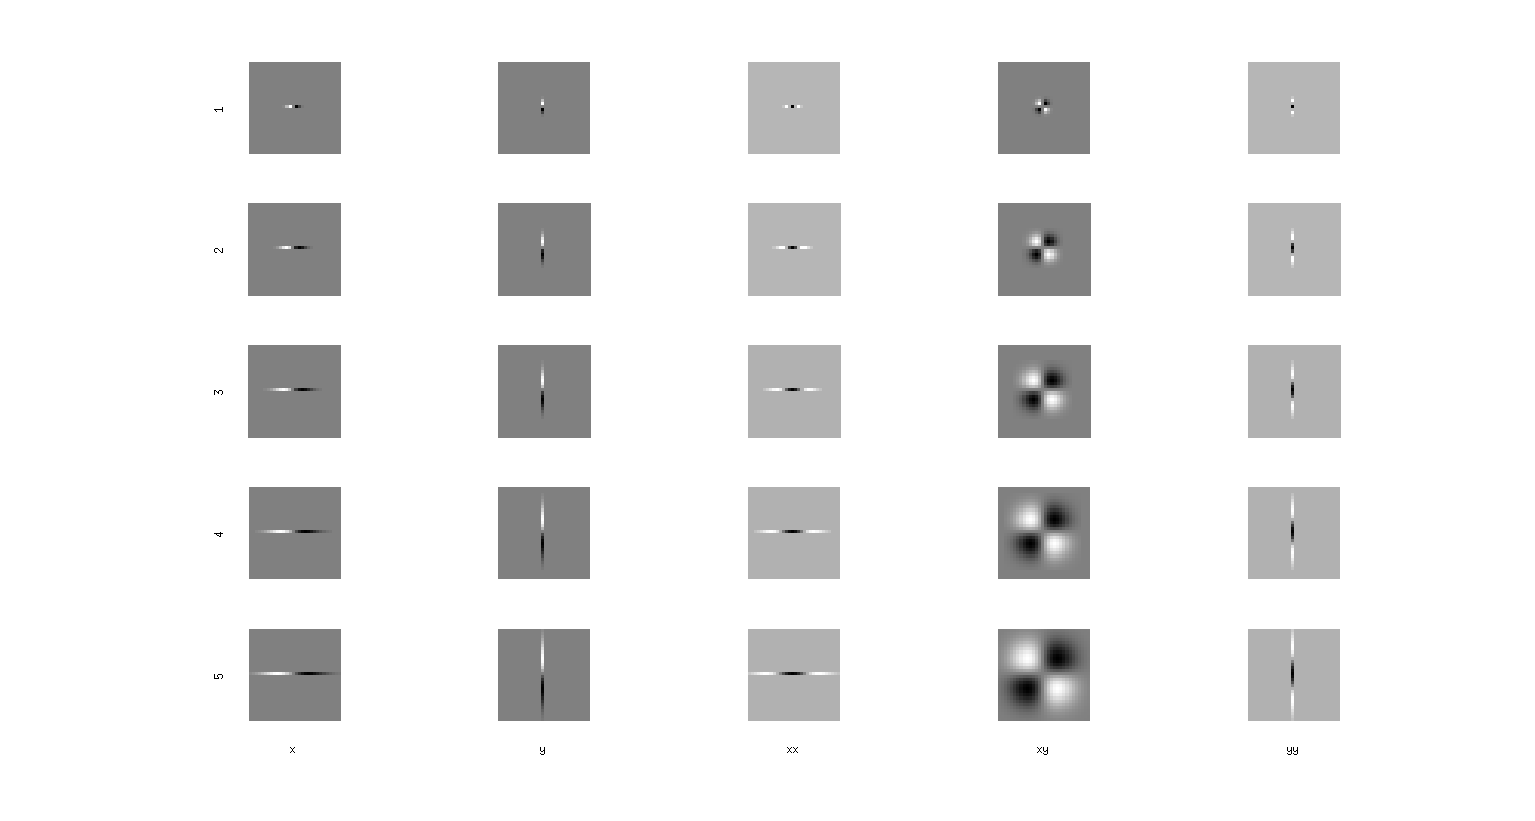
\includegraphics[width=\textwidth]{zebra_img/impulse}
\caption{30x30 impulse image convolved with various filters with $\sigma \in {1,2,3,4,5}$}
\label{fig:impulse}
\end{figure}


\end{document}
